\section{Projet}
\begin{frame}
    \frametitle{\color{white}Projet}
    \begin{block}{Interface graphique : GuiPG}
      \begin{itemize}
        \item Gestion d'un trousseau de clé gpg.
        \item Actions cryptographiques.
        \item Représentation de la toile de confiance.
        \item Visualisation des commandes nécessaire pour chaque actions.
      \end{itemize}
    \end{block}

    \begin{block}{Étude de GnuPG}
    \begin{itemize}
      \item Documentation sur les possibilités de GnuPG.
      \item Guide d'utilisation de GnuPG.
    \end{itemize}
      
    \end{block}
    \begin{block}{Attaque sur les identifiants de clé}
      \begin{itemize}
        \item Forger une 2\up{nd} pré-image d'un clé sur les 4 dernier octets de son identifiant.
        \item Documentation sur les limites de GnuPG.
      \end{itemize}
    \end{block}
\end{frame}

\begin{frame}
  \frametitle{\color{white}Visualisation toile de confiance}
    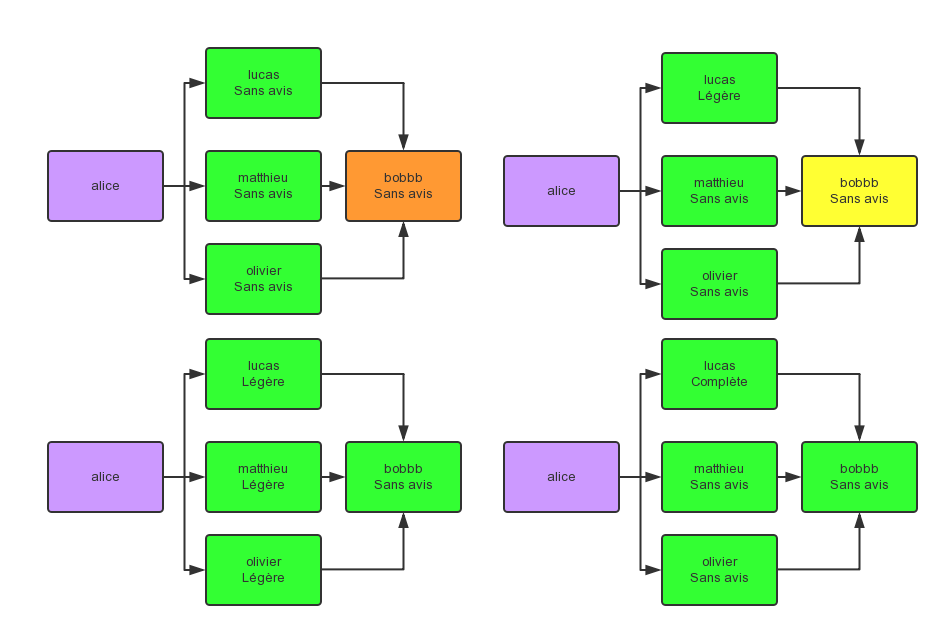
\includegraphics[scale=0.3]{tdcdemo.png}
\end{frame}

\begin{frame}
  \frametitle{\color{white}GuiPG}
  \begin{block}{Gestion d'un trousseau de clé gpg}
      \begin{itemize}
        \item Création de clé / sous clé.
        \item Suppression de clé principale.
        \item Certification de clé.
        \item Modification de la confiance.
        \item Ajouter un identifiant utilisateur.
        \item Importation / Exportation de clés depuis un fichier.
      \end{itemize}
    \end{block}
    \begin{block}{Opérations cryptographique}
      \begin{itemize}
        \item Chiffrer un fichier, pour plusieurs destinataires de façon anonyme ou non.
        \item Déchiffrer un fichier et vérifier les signatures.
      \end{itemize}
    \end{block}
\end{frame}

\begin{frame}
  \frametitle{\color{white}Attaque}
  \begin{block}{Fonctionnement}
      \begin{itemize}
        \item Crée une clef RSA.
        \item Regarde son haché.
        \item Modifie la date de création.
        \item Compare le haché avec celui espéré.
        \item Si le haché obtenu est le bon, création d'une clé avec un KeyId identique à la première.
      \end{itemize}
    \end{block}
\end{frame}

\begin{frame}
  \frametitle{\color{white}Les problèmes de l'attaque}
  \begin{block}{Date de création}
      \begin{itemize}
        \item La date de création doit être supérieure à 1970 l'année 0 dans les machines.
        \item La date de création doit être inférieur à la date d'aujourd'hui.
      \end{itemize}
    \end{block}
    \medbreak
    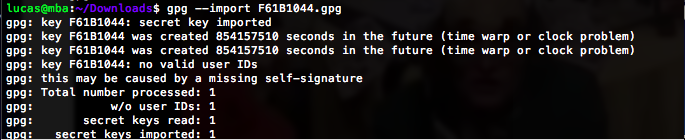
\includegraphics[scale=0.42]{attaque.png}
\end{frame}


\section{Les risques survenus}
  \subsection{Risques organisationnels}
    \begin{frame}
      \frametitle{\color{white}Risques organisationnels}
      \begin{block}{Perte de membres}
        Deux membres ont quitter le projet durant le premier sprint.
      \end{block}
      \begin{block}{Incompatibilité d'emploi du temps}
        Deux membres sont passé en GIL.\\
        Difficultés pour se réunir.
      \end{block}
      \pause
      \begin{exampleblock}{Solutions}
        \begin{itemize}
          \item Mis en place d'un plan d'action
          \item Redéfinition du périmètre du projet
          \item Mise en place d'un créneau hebdomadaire commun.
        \end{itemize}
      \end{exampleblock}
    \end{frame}

  \subsection{Risques techniques}
    \begin{frame}
      \frametitle{\color{white}Maîtrise des outils}
      \begin{block}{Maîtrise des outils}
        Majorité des membres pas assez formé sur les outils utilisé\\
        (git, Qt, C++, gpg)
      \end{block}
      \pause
      \begin{exampleblock}{Solutions}
        \begin{itemize}
          \item Réunion d'installation et de formation aux outils
        \end{itemize}
      \end{exampleblock}
    \end{frame}
    \begin{frame}
      \frametitle{\color{white}Fonctionnement technique de GnuPG}
      \begin{block}{Fonctionnement technique de GnuPG}
        GnuPG utilise directement un tty comme entrée / sortie pour certaine commandes.\\
        Ce qui nous a compliqué la tâche pour arriver a envoyer
        et récupérer des données du logiciel.
      \end{block}
      \pause
      \begin{exampleblock}{Solutions}
        \begin{itemize}
          \item Inspection du code source de GnuPG et de son comportement
          \item Réalisation d'un pseudo-terminal
        \end{itemize}
      \end{exampleblock}
    \end{frame}

\section{Bilan du projet}
  \begin{frame}
    \frametitle{\color{white}Bilan du projet}
    \begin{block}{Axes d'améliorations}
      Améliorations de l'interface GuiPG :
      \begin{itemize}
        \item Affiner la gestion de clé
        \item Ajouter une visualisation sous forme de graphe de la toile de confiance
        \item Personnalisation de l'interface
      \end{itemize}
      Améliorations de l'attaque :
      \begin{itemize}
        \item Paralléliser le calcul des hashs de la clé sur CPU
        \item Implanter l'attaque sur carte graphique (OpenCL, CUDA)
      \end{itemize}
    \end{block}
    
    \begin{block}{Rétrospective}
    Approfondir l'étude de faisabilité lors de la phase d'avant projet.
      \begin{itemize}
        \item Réaliser une étude poussé du logiciel gpg.
        \item S'assurer de la compréhension et de la maîtrise des outils de la part de chacun.
      \end{itemize}
    \end{block}


  \end{frame}
